% 03 — Zadatak 3: formulacija opt. problema, optimalna aproksimacija s ograničenjima.

\section{Zadatak 3 --- optimalna aproksimacija s ograničenjima}
\label{sec:zad3}

\subsection{Opis problema izgradnje ceste na neravnom terenu}
\label{sec:zad3:opis}

Cestu treba izgraditi na neravnom terenu poznate visine $h(x)$, $x \in [0, L]$.
Trošak izrade proporcionalan je količini materijala koju treba otkopati ili
dodati da bi se dobio profil ceste $y(x)$, uz ograničenja na nagib, na brzinu
promjene nagiba te uz zadane rubne uvjete \cite[str.~1]{jokic_zadatak}. Zadano je
\begin{equation}
  L = 10, \qquad h(x) = 0{,}0053x^4 - 0{,}095x^3 + 0{,}48x^2 - 0{,}3x + 1,
\end{equation}
uz $a = h(0) = 1$ i $b = h(L) = 4$, te dva slučaja:
slučaj A s $b_1 = 0{,}5$, $b_2 = 0{,}5$ i slučaj B s $b_1 = 0{,}5$, $b_2 = 0{,}2$.

\subsection{Diskretizacija i aproksimacija derivacija}
\label{sec:zad3:diskretizacija}

Interval $[0,L]$ dijeli se na $N$ podintervala duljine $\Delta x = L/N$, s
čvorovima $x_i = i\,\Delta x$, $i = 0,\dots,N$, pri čemu je $x_0 = 0$ i $x_N = L$.
Nepoznanice su visine ceste u čvorovima, $y_i = y(x_i)$.

Nagib se aproksimira prvom podijeljenom razlikom, a brzina promjene nagiba
ponovnom primjenom iste operacije:
\begin{equation}
  \nabla y_i = \frac{y_i - y_{i-1}}{\Delta x},\quad i = 1,\dots,N, \qquad
  \nabla^2 y_i = \frac{\nabla y_i - \nabla y_{i-1}}{\Delta x}
               = \frac{y_i - 2y_{i-1} + y_{i-2}}{\Delta x^2},\quad i = 2,\dots,N .
  \label{eq:z3diff}
\end{equation}
Obje su aproksimacije \emph{linearne} u nepoznanicama $y_i$, što je ključno za
klasifikaciju problema.

\subsection{Formulacija optimizacijskog problema}
\label{sec:zad3:formulacija}

Količina premještenog materijala na $i$-tom podintervalu proporcionalna je
apsolutnoj razlici visina, jer se i otkopavanje i nasipavanje jednako plaćaju.
Ukupni trošak je stoga
\begin{equation}
  J(y) = \sum_{i=0}^{N} \lvert y_i - h(x_i)\rvert \,\Delta x,
  \label{eq:z3cost}
\end{equation}
što je diskretizacija integrala $\int_0^L |y(x)-h(x)|\,\mathrm{d}x$, dakle
$\ell_1$ norma odstupanja. Problem glasi
\begin{align}
  \min_{y \in \mathbb{R}^{N+1}}\quad & \sum_{i=0}^{N} \lvert y_i - h_i\rvert\,\Delta x \label{eq:z3a}\\
  \text{uz}\quad & \lvert y_i - y_{i-1}\rvert \le b_1 \Delta x, && i = 1,\dots,N, \label{eq:z3b}\\
                 & \lvert y_i - 2y_{i-1} + y_{i-2}\rvert \le b_2 \Delta x^2, && i = 2,\dots,N, \label{eq:z3c}\\
                 & y_0 = a, \quad y_N = b . \label{eq:z3d}
\end{align}

\subsection{Klasifikacija problema}
\label{sec:zad3:klasa}

Funkcija cilja \eqref{eq:z3a} je konveksna ali nije glatka, dok su sva
ograničenja linearna. Standardnom \emph{epigrafskom reformulacijom} uvode se
pomoćne varijable $t_i$ uz
\begin{equation}
  y_i - h_i \le t_i, \qquad -(y_i - h_i) \le t_i,
\end{equation}
što je ekvivalentno $t_i \ge |y_i - h_i|$, a cilj postaje $\sum_i t_i \Delta x$.
Time i cilj i sva ograničenja postaju linearni, pa je riječ o
\textbf{linearnom programu} (LP) \cite[str.~30]{jokic_lpqp} s $2(N+1)$ varijabli.
Apsolutne vrijednosti u \eqref{eq:z3b}--\eqref{eq:z3c} razlažu se na po dvije
linearne nejednakosti na isti način.

Da je trošak bio proporcionalan \emph{kvadratu} odstupanja, problem bi bio QP;
$\ell_1$ mjera je ovdje fizikalno ispravna jer je količina zemlje razmjerna
apsolutnoj, a ne kvadriranoj razlici. Ta razlika ima i praktičnu posljedicu:
$\ell_1$ cilj daje rješenja koja se na dijelovima \emph{točno} poklapaju s
terenom, dok bi $\ell_2$ cilj odstupanje razmazao po cijeloj domeni.

\subsection{Rezultati}
\label{sec:zad3:rezultati}

Problem je riješen funkcijom \texttt{linprog} za sva četiri tražena slučaja.
Svi su riješeni do optimalnosti; rezultati su u tablici~\ref{tab:z3}, a profili
na slici~\ref{fig:z3}.

\begin{table}[htbp]
  \centering
  \caption{Rezultati za četiri slučaja. Aktivna ograničenja pokazuju koje
  ograničenje oblikuje rješenje.}
  \label{tab:z3}
  \begin{tabular}{llccccc}
    \hline
    Slučaj & $N$ & $b_1$ & $b_2$ & trošak & aktivnih nagiba & aktivnih zakrivljenosti \\
    \hline
    A & $20$  & $0{,}5$ & $0{,}5$ & $1{,}916180$ & $10/20$  & $3/19$  \\
    A & $100$ & $0{,}5$ & $0{,}5$ & $1{,}965940$ & $51/100$ & $35/99$ \\
    B & $20$  & $0{,}5$ & $0{,}2$ & $2{,}453727$ & $5/20$   & $12/19$ \\
    B & $100$ & $0{,}5$ & $0{,}2$ & $2{,}506047$ & $25/100$ & $73/99$ \\
    \hline
  \end{tabular}
\end{table}

\begin{figure}[htbp]
  \centering
  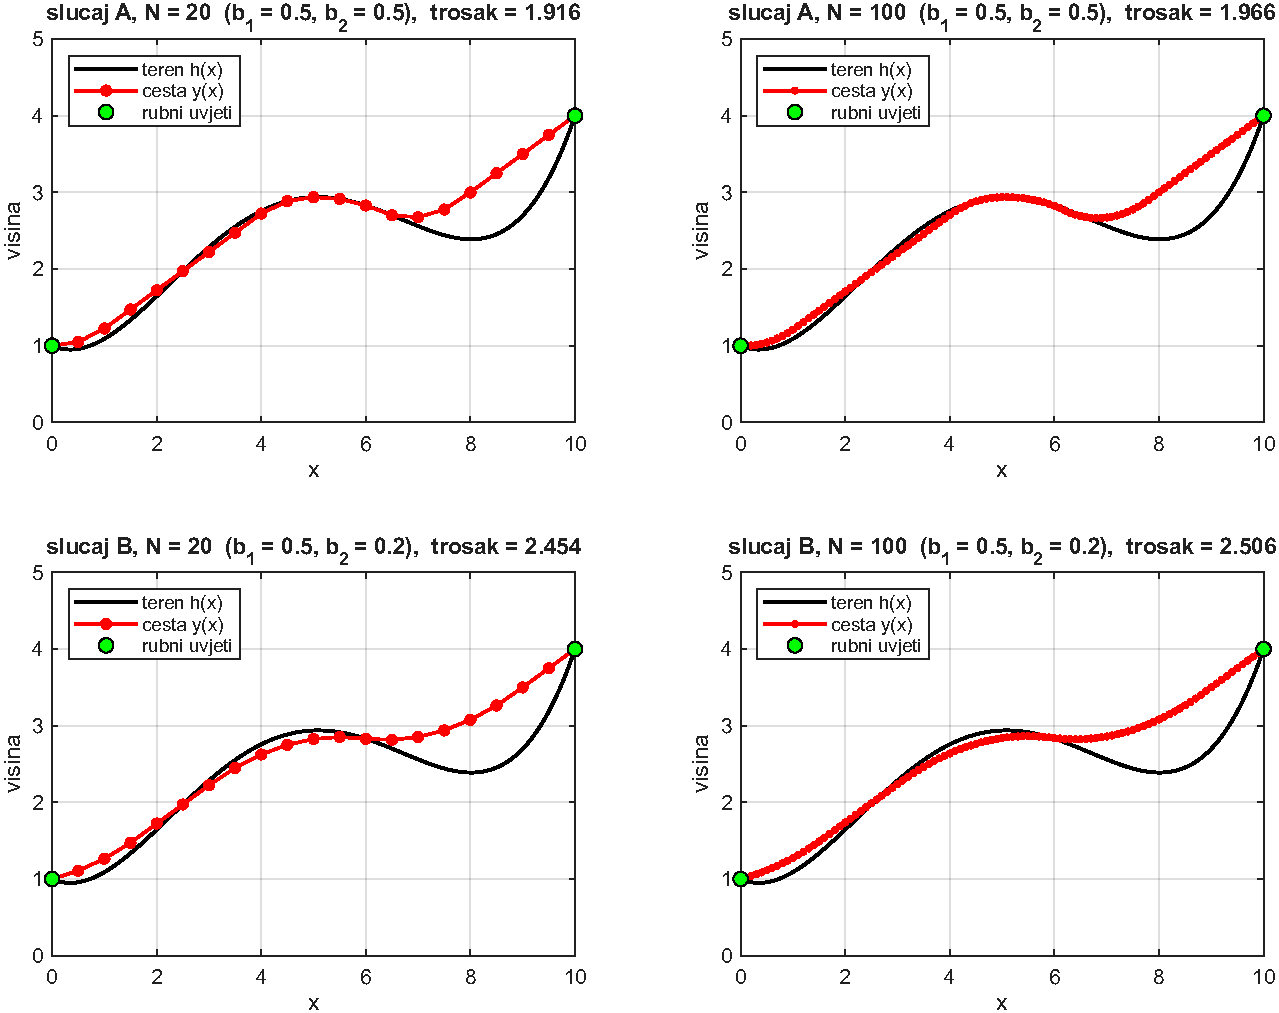
\includegraphics[width=\textwidth]{figures/zad3_cesta.pdf}
  \caption{Teren $h(x)$ (crno) i optimalni profil ceste $y(x)$ (crveno) za sva
  četiri slučaja. Zelene točke su rubni uvjeti.}
  \label{fig:z3}
\end{figure}

U svim slučajevima rubni uvjeti su zadovoljeni do strojne točnosti, a
ograničenja \eqref{eq:z3b}--\eqref{eq:z3c} dosegnuta su točno na svojim
granicama ($\max|\nabla y| = 0{,}5$, $\max|\nabla^2 y| = b_2$), što potvrđuje da
su ona doista aktivna i da rješenje leži na rubu dozvoljenog skupa.

\subsection{Usporedba slučajeva i utjecaj diskretizacije}
\label{sec:zad3:diskusija}

\paragraph{Utjecaj ograničenja $b_2$.} Slučaj B je stroži i skuplji: trošak raste
s $1{,}92$ na $2{,}45$ pri $N=20$, dakle za oko $28\,\%$. Struktura rješenja se
kvalitativno mijenja --- u slučaju A dominira ograničenje nagiba (aktivno na
polovici čvorova), dok u slučaju B prevladava ograničenje zakrivljenosti
($73/99$ aktivnih pri $N=100$). Profil u slučaju B je vidljivo glađi jer se
nagib ne smije mijenjati brzo, pa cesta ne može tako vjerno pratiti teren.

\paragraph{Utjecaj diskretizacije.} Prijelaz s $N=20$ na $N=100$ mijenja trošak
tek u trećoj znamenki ($1{,}916 \to 1{,}966$ i $2{,}454 \to 2{,}506$, oko
$2\,\%$). Rješenje dakle konvergira i grubljom mrežom već je dobro
aproksimirano. Blagi porast je očekivan: finija mreža bolje aproksimira integral
i uz to nameće ograničenja u više točaka, pa je dozvoljeni skup nešto uži.

\paragraph{Oblik rješenja.} Na dijelovima gdje teren zadovoljava ograničenja
cesta ga prati gotovo točno, čime je trošak lokalno nula. Odstupanje se
koncentrira ondje gdje teren mijenja smjer prebrzo --- osobito u udolini oko
$x \approx 8$, gdje teren pada, a cesta mora nastaviti rasti kako bi dosegla
rubni uvjet $y(L) = 4$ uz ograničen nagib. Upravo taj dio nosi najveći dio
troška i u oba slučaja određuje rješenje.
